\clearpage
\subsection{Direction determination}
In this section different methods of determining the direction of the drone is researched. 

\subsubsection{Optical Tracking}
It is possible to position an object precisely using an optical sensor. Though because of weather related issues optical tracking of a drone might not be a functional solution. 
\todo[author=Alexander]{Expand optical tracking section.}


\subsubsection{\glsentrylong{aoa} determination from signal distance difference}








\subsubsection{Phase difference detection}
The \gls{doa} of a signal can be determined by measuring the phase difference of the signal at two antennas spaced apart.
The drone will need to send out a beacon signal and two antennas on the ground will have to measure the phase difference of the signal. 

\begin{figure}[h]
\centering
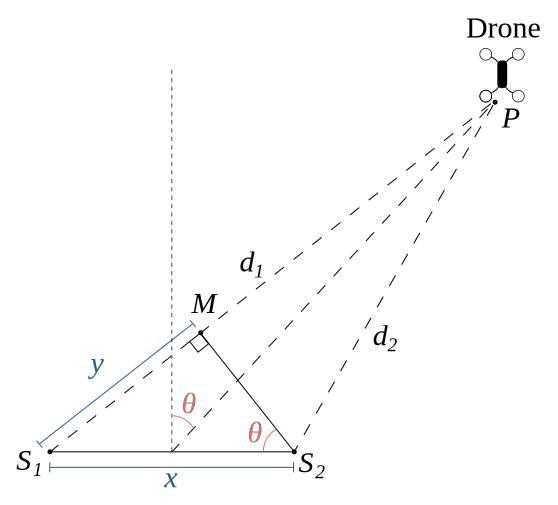
\includegraphics[width=0.7\linewidth]{Phase/Phase_drawing}
\caption{Illustration of determination of \gls{aoa} using the phase difference. P is the point where the drone is located. $d_1$ and $d_2$ are the respective distances between the drone and the two receiving antennas $S_1$ and $S_2$. The distance between the antennas is $x$ and the difference in $d2$ and $d_1$ is y. $M$ denotes the point where the two distances are equal. The \gls{aoa} is $\theta$ when approximating that $d_1 \gg x$ and $d_2 \gg x$.}
\label{fig:phase_drawing}
\end{figure}


The formula for determining the \gls{aoa} can be derived using geometry.
Consider a signal sent from the drone at point $P$ on \autoref{fig:phase_drawing}. Two antennas are placed at respectively at $S_1$ and $S_2$. The paths that the signals travel to reach the two antennas are $d_1$ and $d_2$. At the point $M$ the two signals have travelled the same distance and thus have the same phase. 
The difference of length is denoted $y$ and is equal to $d_2-d_1$. This distance can be expressed by:
\begin{equation} \label{eq:phasedaoay}
y=\frac{\lambda\cdot\Delta\varphi}{2\pi}
\end{equation}
\startexplain
\explain{$\lambda$ is the wavelength of the signal}{\si{\meter}}
\explain{$\Delta\varphi$ is the phase difference of the signal between the two antennas}{\si{\radian}}
\stopexplain

When isolating for $\Delta\varphi$ the equation becomes
\begin{equation}
\Delta\varphi=y\frac{2\pi}{\lambda}
\end{equation}
In practice when measuring the phase difference of two signals it falls in the interval: $-\pi<\Delta\varphi<\pi$. Therefore it can be seen from \autoref{eq:phasedaoay}, that $x$ must fall in the interval $\frac{-\lambda}{2} < y < \frac{\lambda}{2}$. This means that the maximum possible distance between the antennas should be $\frac{\lambda}{2}$ to avoid phase ambiguity \citep{TechReport:DirectionFindingPaper,TechReport:Amundson2010}. The maximum phase difference will occur when the sender is located collinear with the receiver. If the \gls{aoa} is directly above the two receiving antennas, the phase difference will be zero degrees.

The \gls{aoa}, $\theta$, can be calculated using trigonometry. We assume that the sender $P$ is so far away that the two lines, $d_1$ and $d_2$, can be considered parallel.
This means that the angle $\theta$ at $S_2$ also becomes the \gls{aoa} which can be calculated using sine \citep{TechReport:DirectionFindingPaper}.

\begin{subequations}
	\begin{align}
	\sin(\theta) = \frac{y}{x} \\
	\theta = \sin^{-1}(\frac{y}{x}) \\
	\theta = \sin^{-1}(\frac{\frac{\lambda\cdot\Delta\varphi}{2\pi}}{x}) \\
	\theta = \sin^{-1}(\frac{\lambda\cdot\Delta\varphi}{2\pi x})
	\end{align}
\end{subequations}
\startexplain
\explain{$\theta$ is the direction of the drone}{\si{\radian}}
\explain{$\lambda$ is the wavelength}{\si{\meter}}
\explain{$\Delta\varphi$ is the phase difference}{\si{\radian}}
\explain{$x$ is the distance between the antennas}{\si{\meter}}
\stopexplain

The method described above will only be able to measure \gls{aoa} within a \SI{180}{\degree} field of view since two mirrored points will result in the same phase difference. 
This can be seen on \autoref{fig:phase_double}. To avoid this ambiguity, the phase has to be measured at more then two receivers \citep{TechReport:Amundson2010}. In this report for the sake of simplicity only a two antenna setup will be considered.

\begin{figure} [h]
\centering
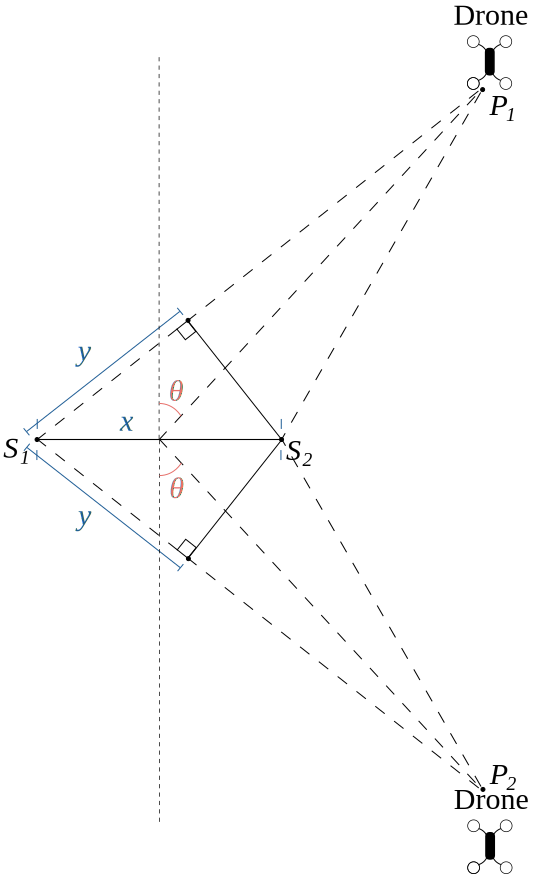
\includegraphics[width=0.4\linewidth]{Phase/phase_double}
\caption{The two points $P_1$ and $P_2$ will result in the same phase difference being measured at the receivers $S_1$ and $S_2$. This means that a two antenna system will only have a field of view of \SI{180}{\degree}}.
\label{fig:phase_double}
\end{figure}


Errors in the \gls{doa} reading ($\Delta\theta '$) occurs depending on the S/N ratio of the signal and is given by \citep[p. 43]{book:shinohara}:
\begin{equation} \label{doasnerror}
\Delta\theta ' = \frac{\lambda}{\pi x \cos(\varphi \sqrt{SN})} 
\end{equation}

\startexplain
\explain{$\Delta\theta '$ is the error of \gls{doa} estimation}{\si{\radian}}
\explain{$x$ is the spacing between the two receiving antennas}{\si{meter}}
\explain{$\theta$ is the estimated \gls{aoa}.}{\si{\radian}}
\explain{$SN$ is the signal to noise ratio}{\si{\decibel}}
\stopexplain

The S/N ratio will decrease when more antennas are used and therefore precise \gls{doa} estimations are made with an array of receivers \citep{book:shinohara}.

\subsubsection{Signal strength difference}
Assuming the drone is transmitting a pilot signal, 
a straightforward way to locate and track the drone is to measure the signal strength of the pilot signal in an array of receivers. This is known as \gls{rssi} tracking. \autoref{fig:RSSI_tracking} shows one example of how this can be done. The targeted object wanting to be tracked emits a pilot wave. The difference in received signal strength between the two tracking antennas is treated as an error signal in a feedback loop controlling the position of the antenna arrays. When the signal strength is equal on both sides of the main antenna, the main antenna is pointing directly at the target.

\begin{figure}[h]
	\centering
	\includegraphics[width=0.8\linewidth]{RSSI_tracking}
	\caption[Placement of tracking antennas in a \gls{rssi} tracking system]{}
	\label{fig:RSSI_tracking}
\end{figure}

This method is simple and precise enough for many uses. However to increase the precision many factors have to be considered, including directionality of the tracking antennas and gain difference between the antennas. 

\subsubsection{\glsentrylong{toa}}
The \gls{toa} method uses the time difference in reception of a source between two receivers. The finite speed of electromagnetic wave propagation causes a time difference between the reception time on two antennas when the signal source is not placed at exactly the same distance to each antenna.

In the case of tracking a drone, the drone carries a pulsing signal source. The two antennas are placed at a known distance from each other, and the drone sends a pulse.
At the times $\tau_1$ and $\tau_2$ the first and second antenna receives the signal respectively. The difference between $\tau_1$ and $\tau_2$ multiplied with the speed of light represents is difference in distance between the drone and the two antennas.

\begin{figure} [h]
	\centering
	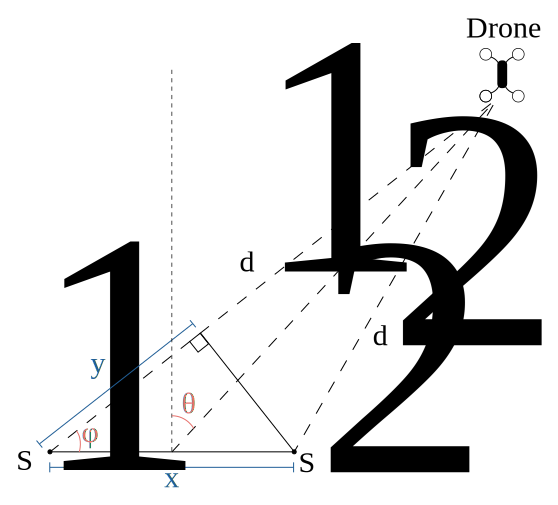
\includegraphics[width=0.9\linewidth]{TOA/ToA_drawing}
	\caption{Illustration of the \gls{toa} method to determine \gls{aoa}. $x$ is the distance between the antennas $S_1$ and $S_2$, $d_1$ and $d_2$ are the distances between the drone and the respective receivers and $y$ is the difference between $d_1$  and $d_2$. $\theta$ represents the angle between the midway point of the antennas and the drone. For $d_1 \gg x$ and $d_2 \gg x$ the angle $\theta$ can be approximated to $\theta \approxeq \varphi$}\label{fig:tech_ToAmethod}
\end{figure}

\autoref{fig:tech_ToAmethod} shows an illustration of this concept. Using trigonometry it is possible to find the angle $\theta$. Assuming the distance to the drone from the antennas is much longer than the distance between the two antennas \autoref{eq:tech_ToA} is used to calculate $\theta$.
\begin{subequations} \label{eq:tech_ToA}
	\begin{align}
		\varphi = \cos^{-1} \left( \frac{y}{x} \right) \addunit{\radian} \\
		y = \Delta \tau \cdot c \addunit{\meter} \\
		\theta \approxeq \SI{90}{\degree} - \varphi \addunit{\radian} \\
		\theta \approxeq \SI{90}{\degree} - \cos^{-1} \left( \frac{ \Delta\tau \cdot c}{x} \right) \addunit{\radian} \\
  		\theta \approxeq \sin^{-1} \left( \frac{ \Delta\tau \cdot c}{x} \right) \addunit{\radian}
	\end{align}
\end{subequations}
\startexplain
\explain{$\theta$ is the angle between the specified forward direction and the location for the drone}{\si{\radian}}
\explain{$x$ is the distance between the receivers}{\si{\meter}}
\explain{$c$ is the speed of light}{\si{\m/s}}
\explain{$\Delta \tau$ is the time difference between the two antennas reception of the signal}{\si{\second}}
\stopexplain


If the difference in time is not registered and measured correctly the calculated angle deviate. From equation \eqref{eq:TOA:eq2}, the allowed error in the measured time of arrival relative to the angular deviation can be calculated. 

\begin{align}\label{eq:TOA:eq2}
\theta_{error} = 90\degree - \cos^{-1} ( \frac{ \tau_{error} \cdot c }{x} ) \nonumber \\
\tau_{error} = \frac{\cos(\theta_{error} - 90\degree) \cdot x}{c} \addunit{\second}
\end{align}
\startexplain
\explain{$\theta_{error}$ is the allowed angular deviation}{\si{\radian}}
\explain{$x$ is the distance between the receivers}{\si{\meter}}
\explain{$c$ is the speed of light}{\si{\m/s}}
\explain{$\tau_{error}$ is the error in time of arrival difference}{\si{\second}}
\stopexplain

\todo[author=Alexander]{We previously found an approximate for the angular deviation, use this as an argument}

\todo[author=Alexander]{Conclusion of the ToA method}
Conclusion of this method
